\chapter{Evaluation on Raspberry Pi CPU}
The following figures are the confusion matrices evaluation on PC CPU.

\begin{figure}[!h]
    \centering
    \subfloat[][RN50]{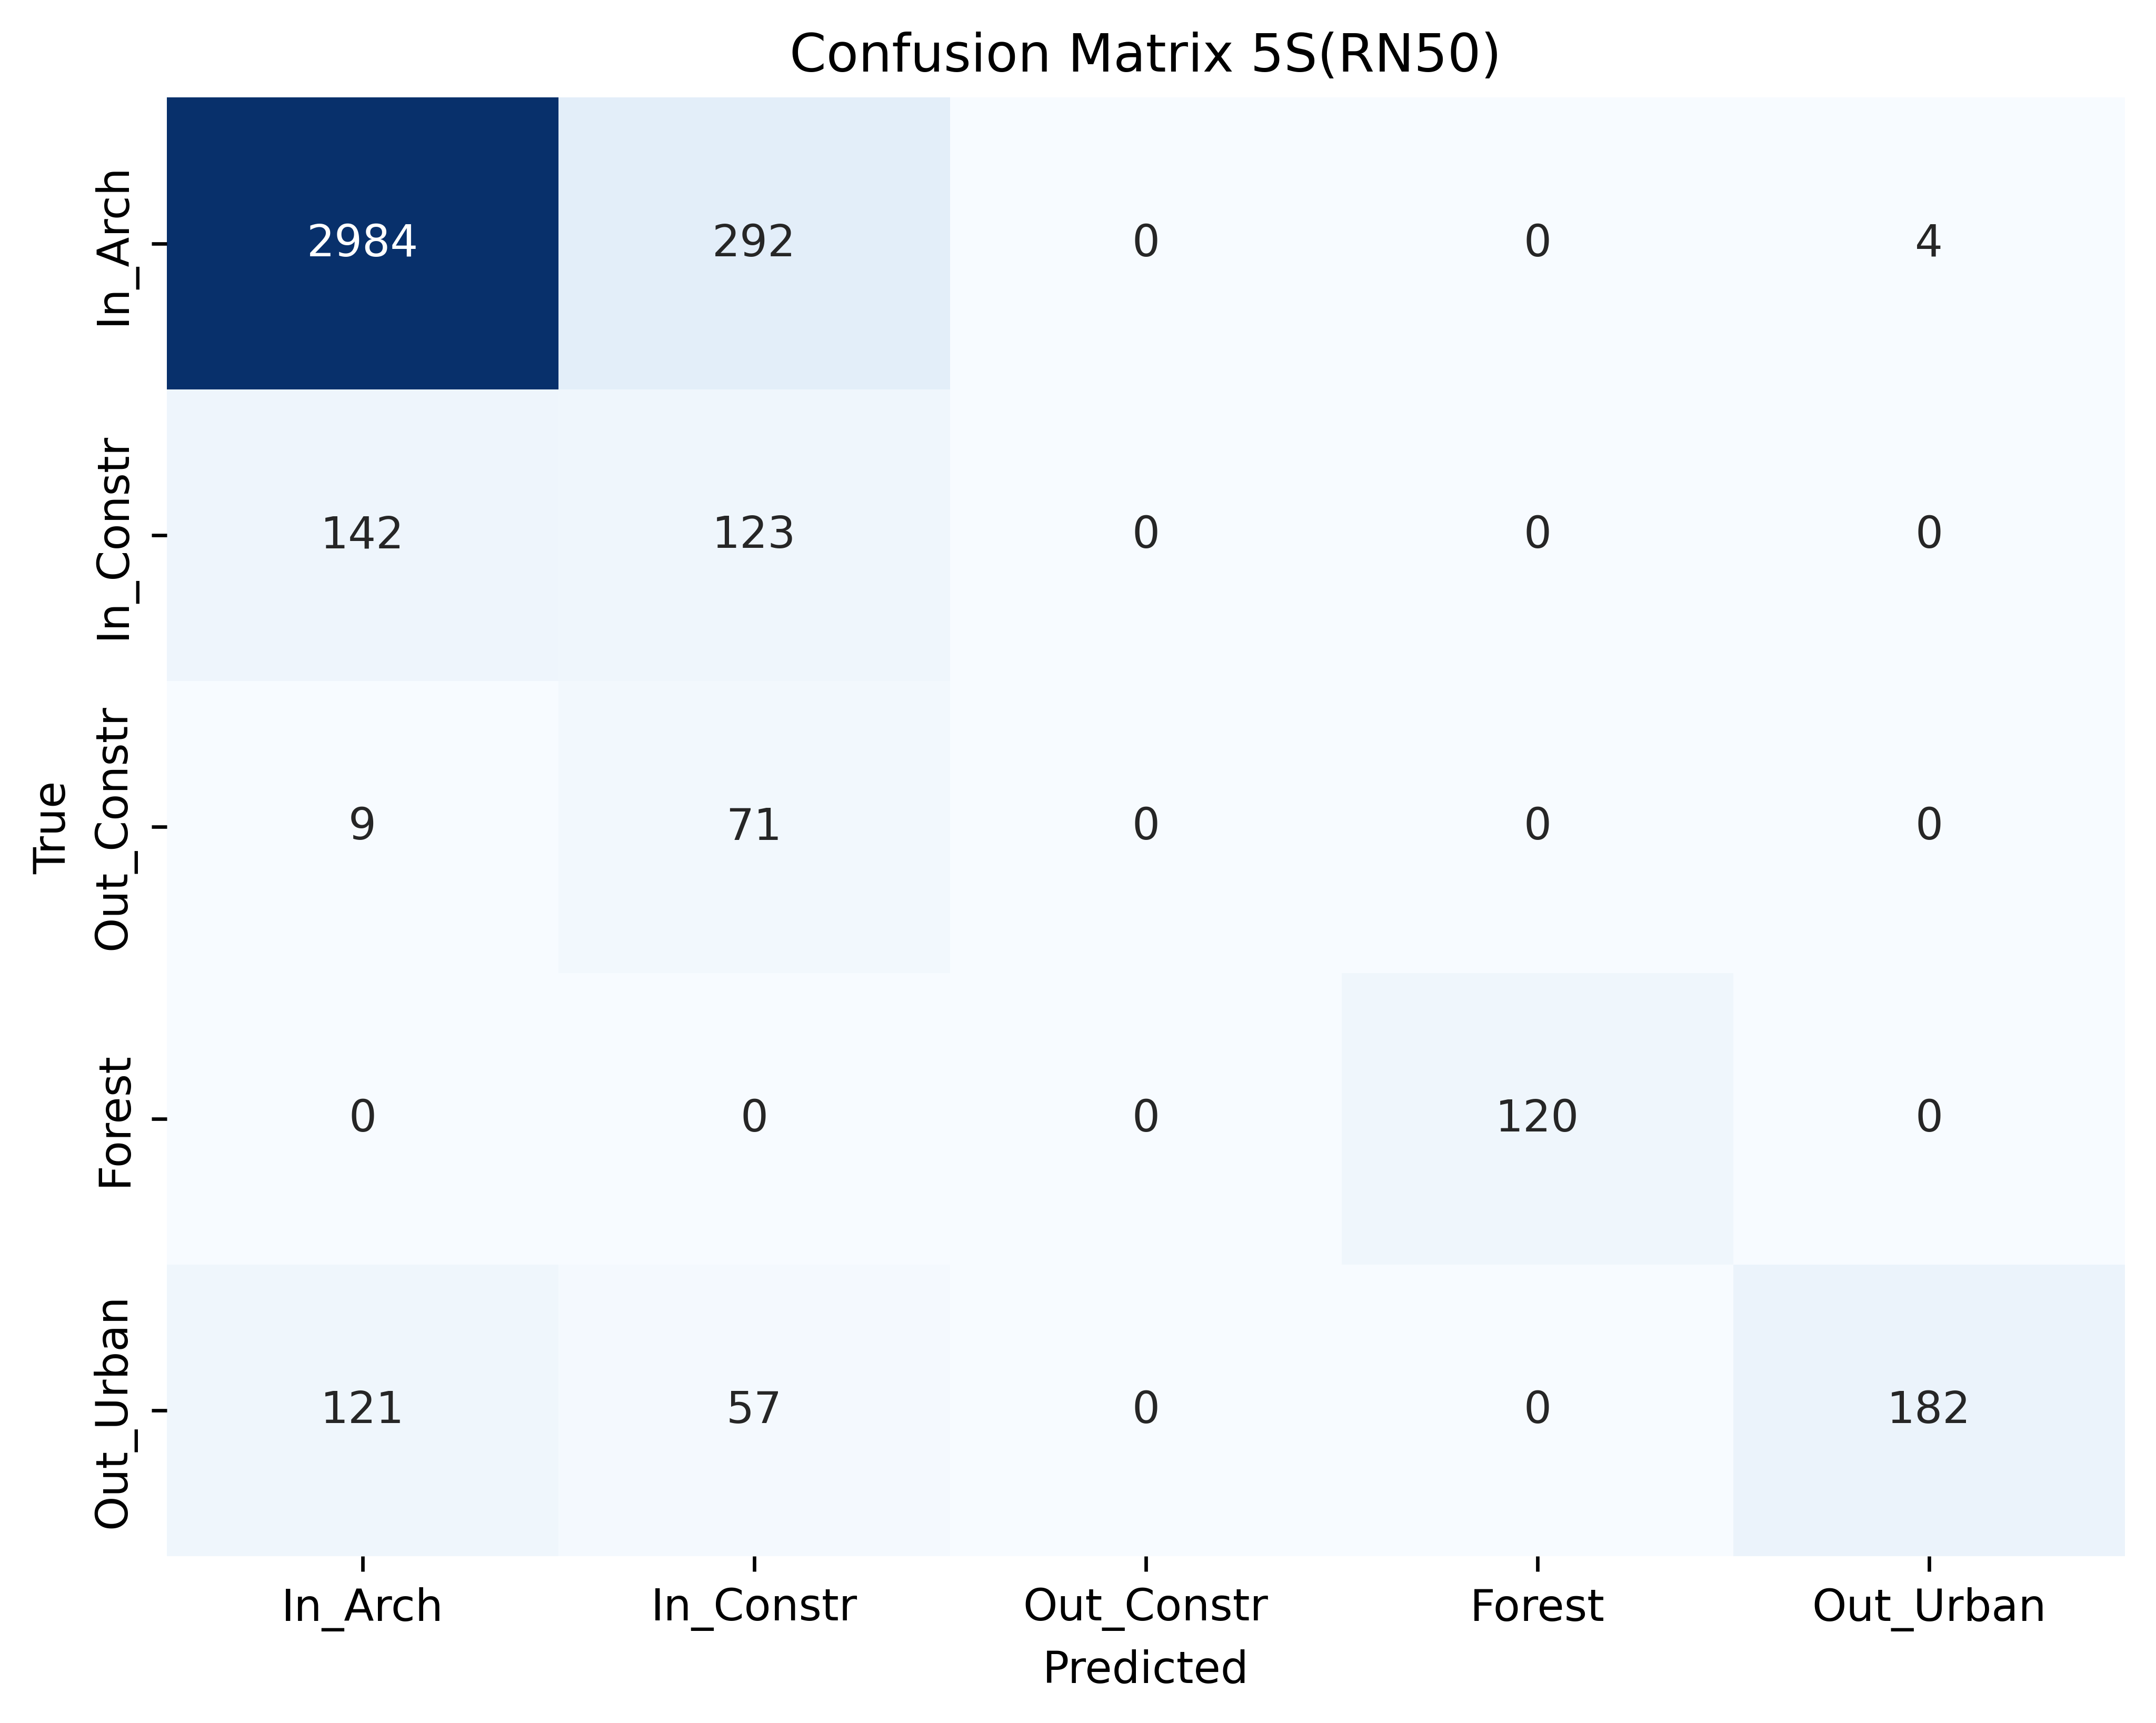
\includegraphics[width=0.45\textwidth]{Images/appendix/resultsRaspi/Confusion Matrix 5S(RN50).png}\label{resultpc:fig:rn505s}}
    \subfloat[][RN50x4]{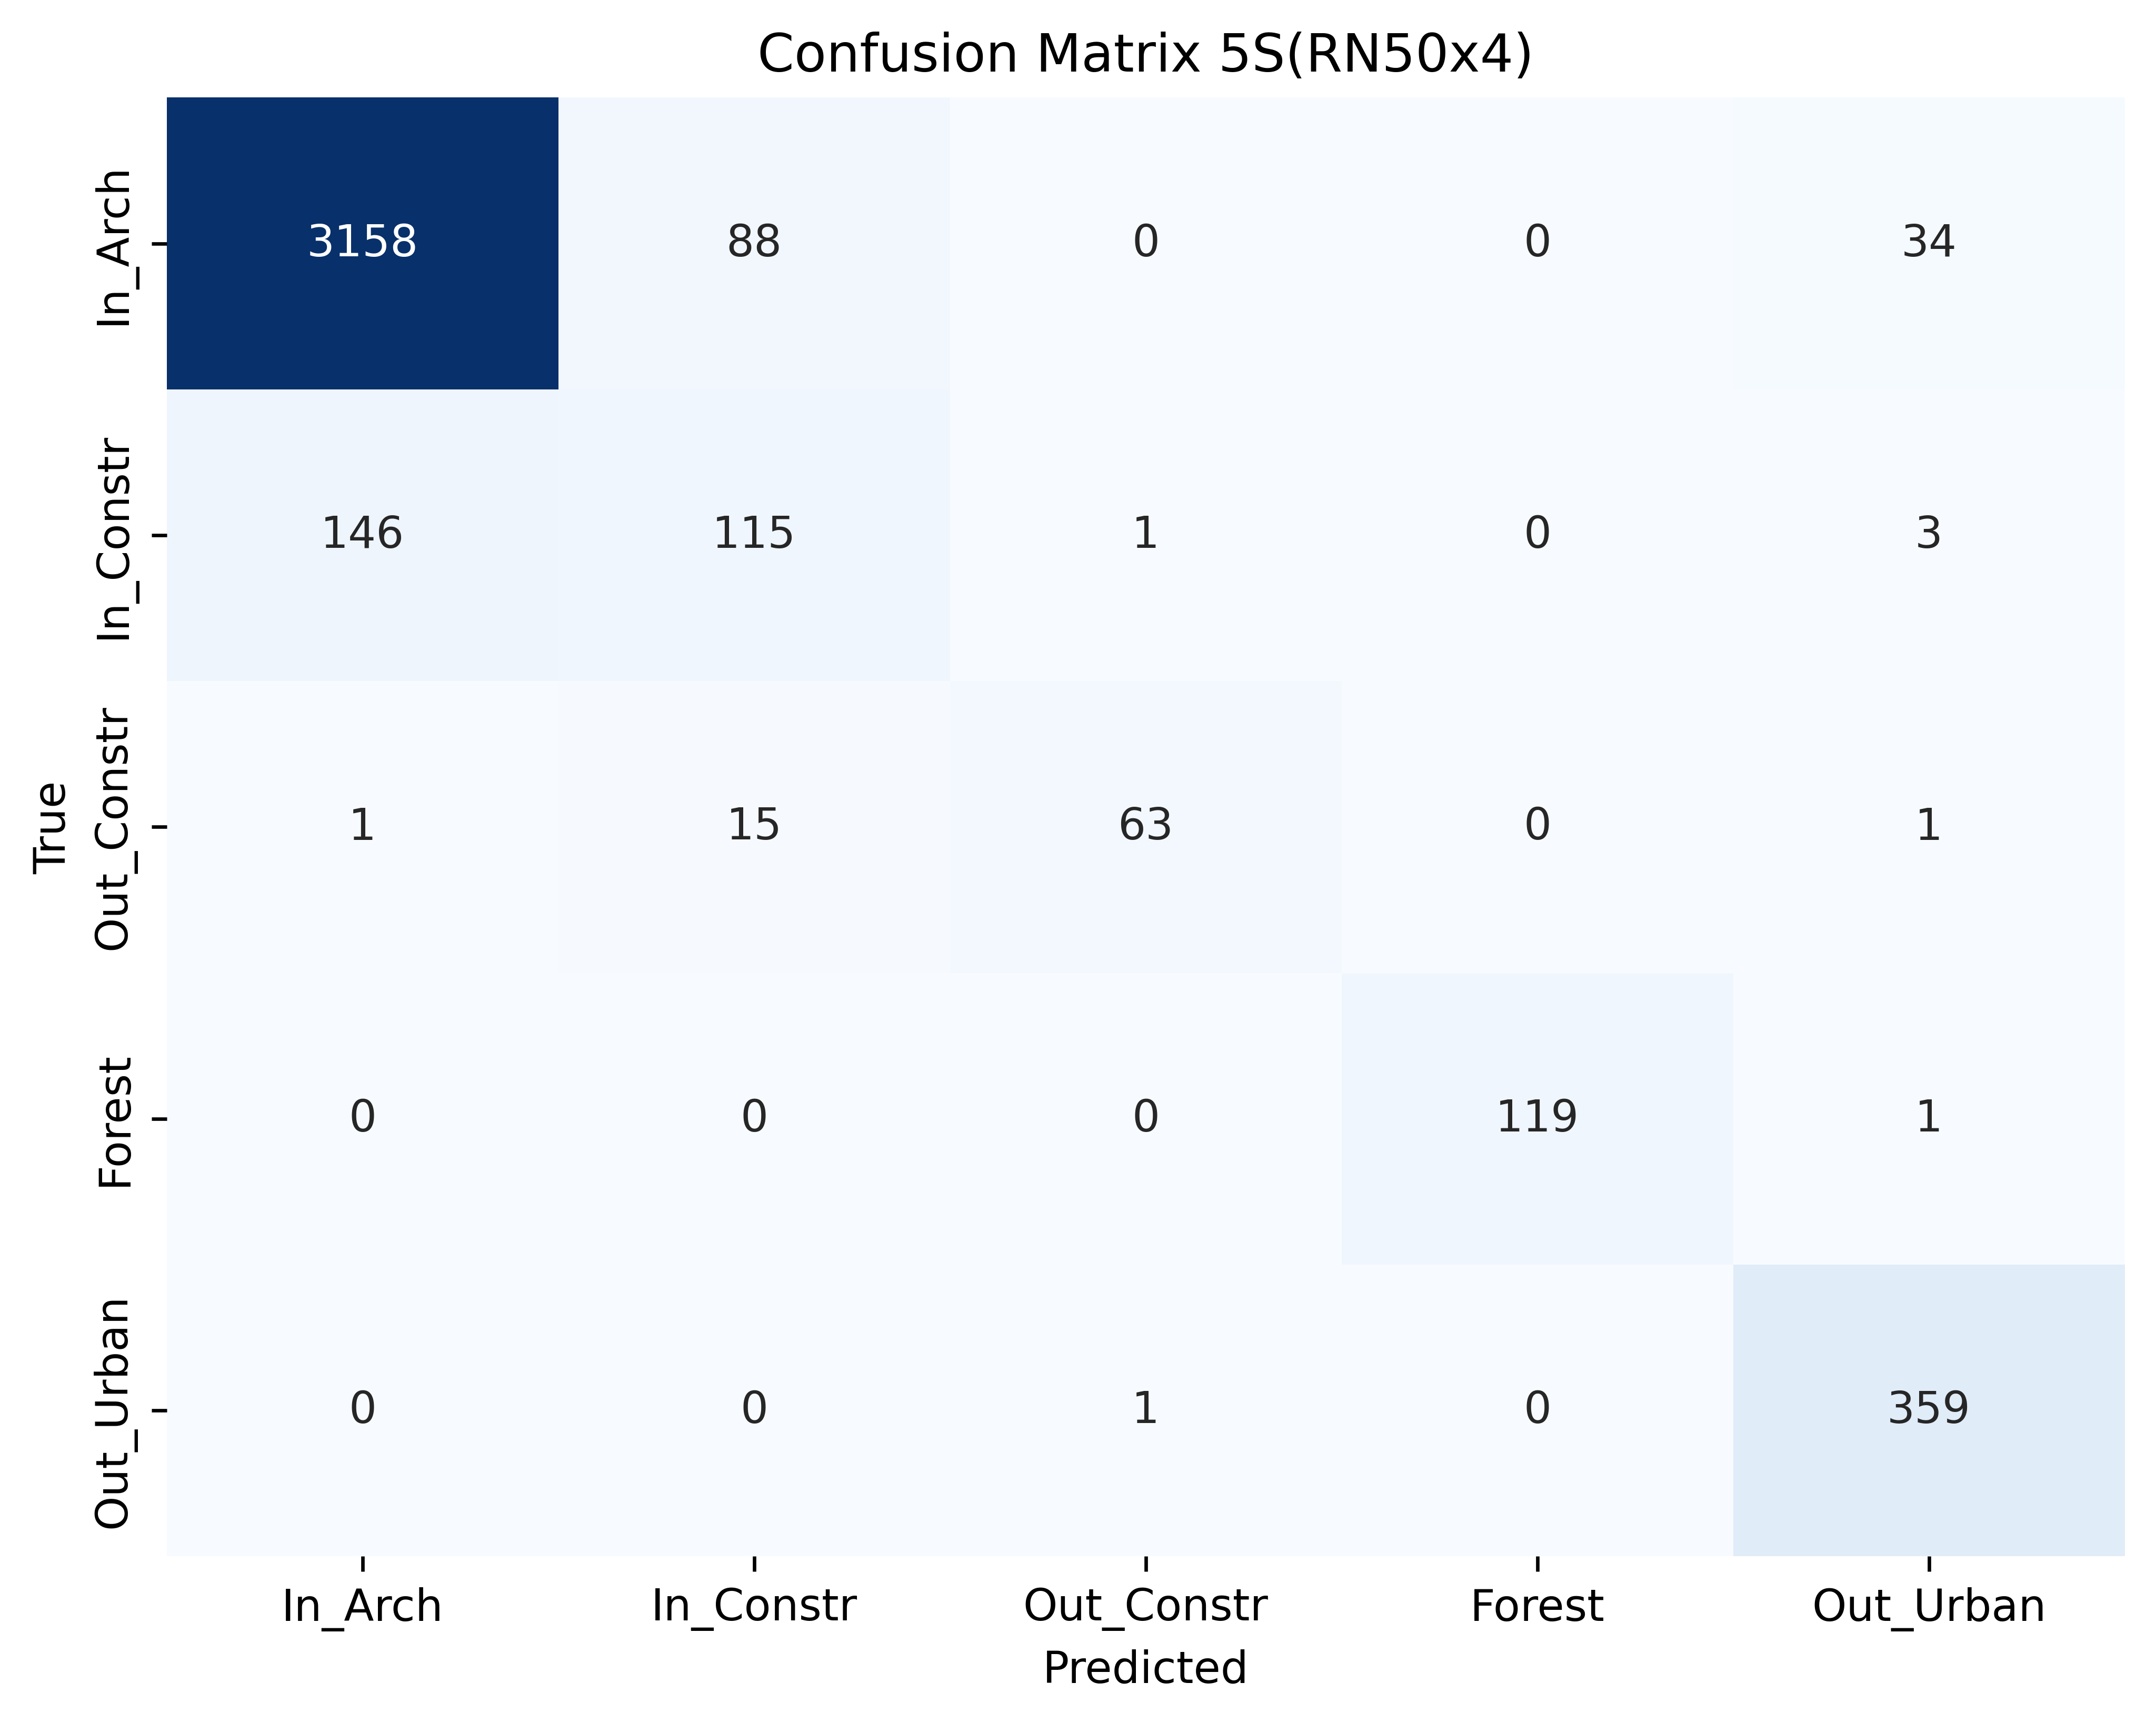
\includegraphics[width=0.45\textwidth]{Images/appendix/resultsRaspi/Confusion Matrix 5S(RN50x4).png}\label{resultpc:fig:rn50x45s}} \\
    \subfloat[][RN101]{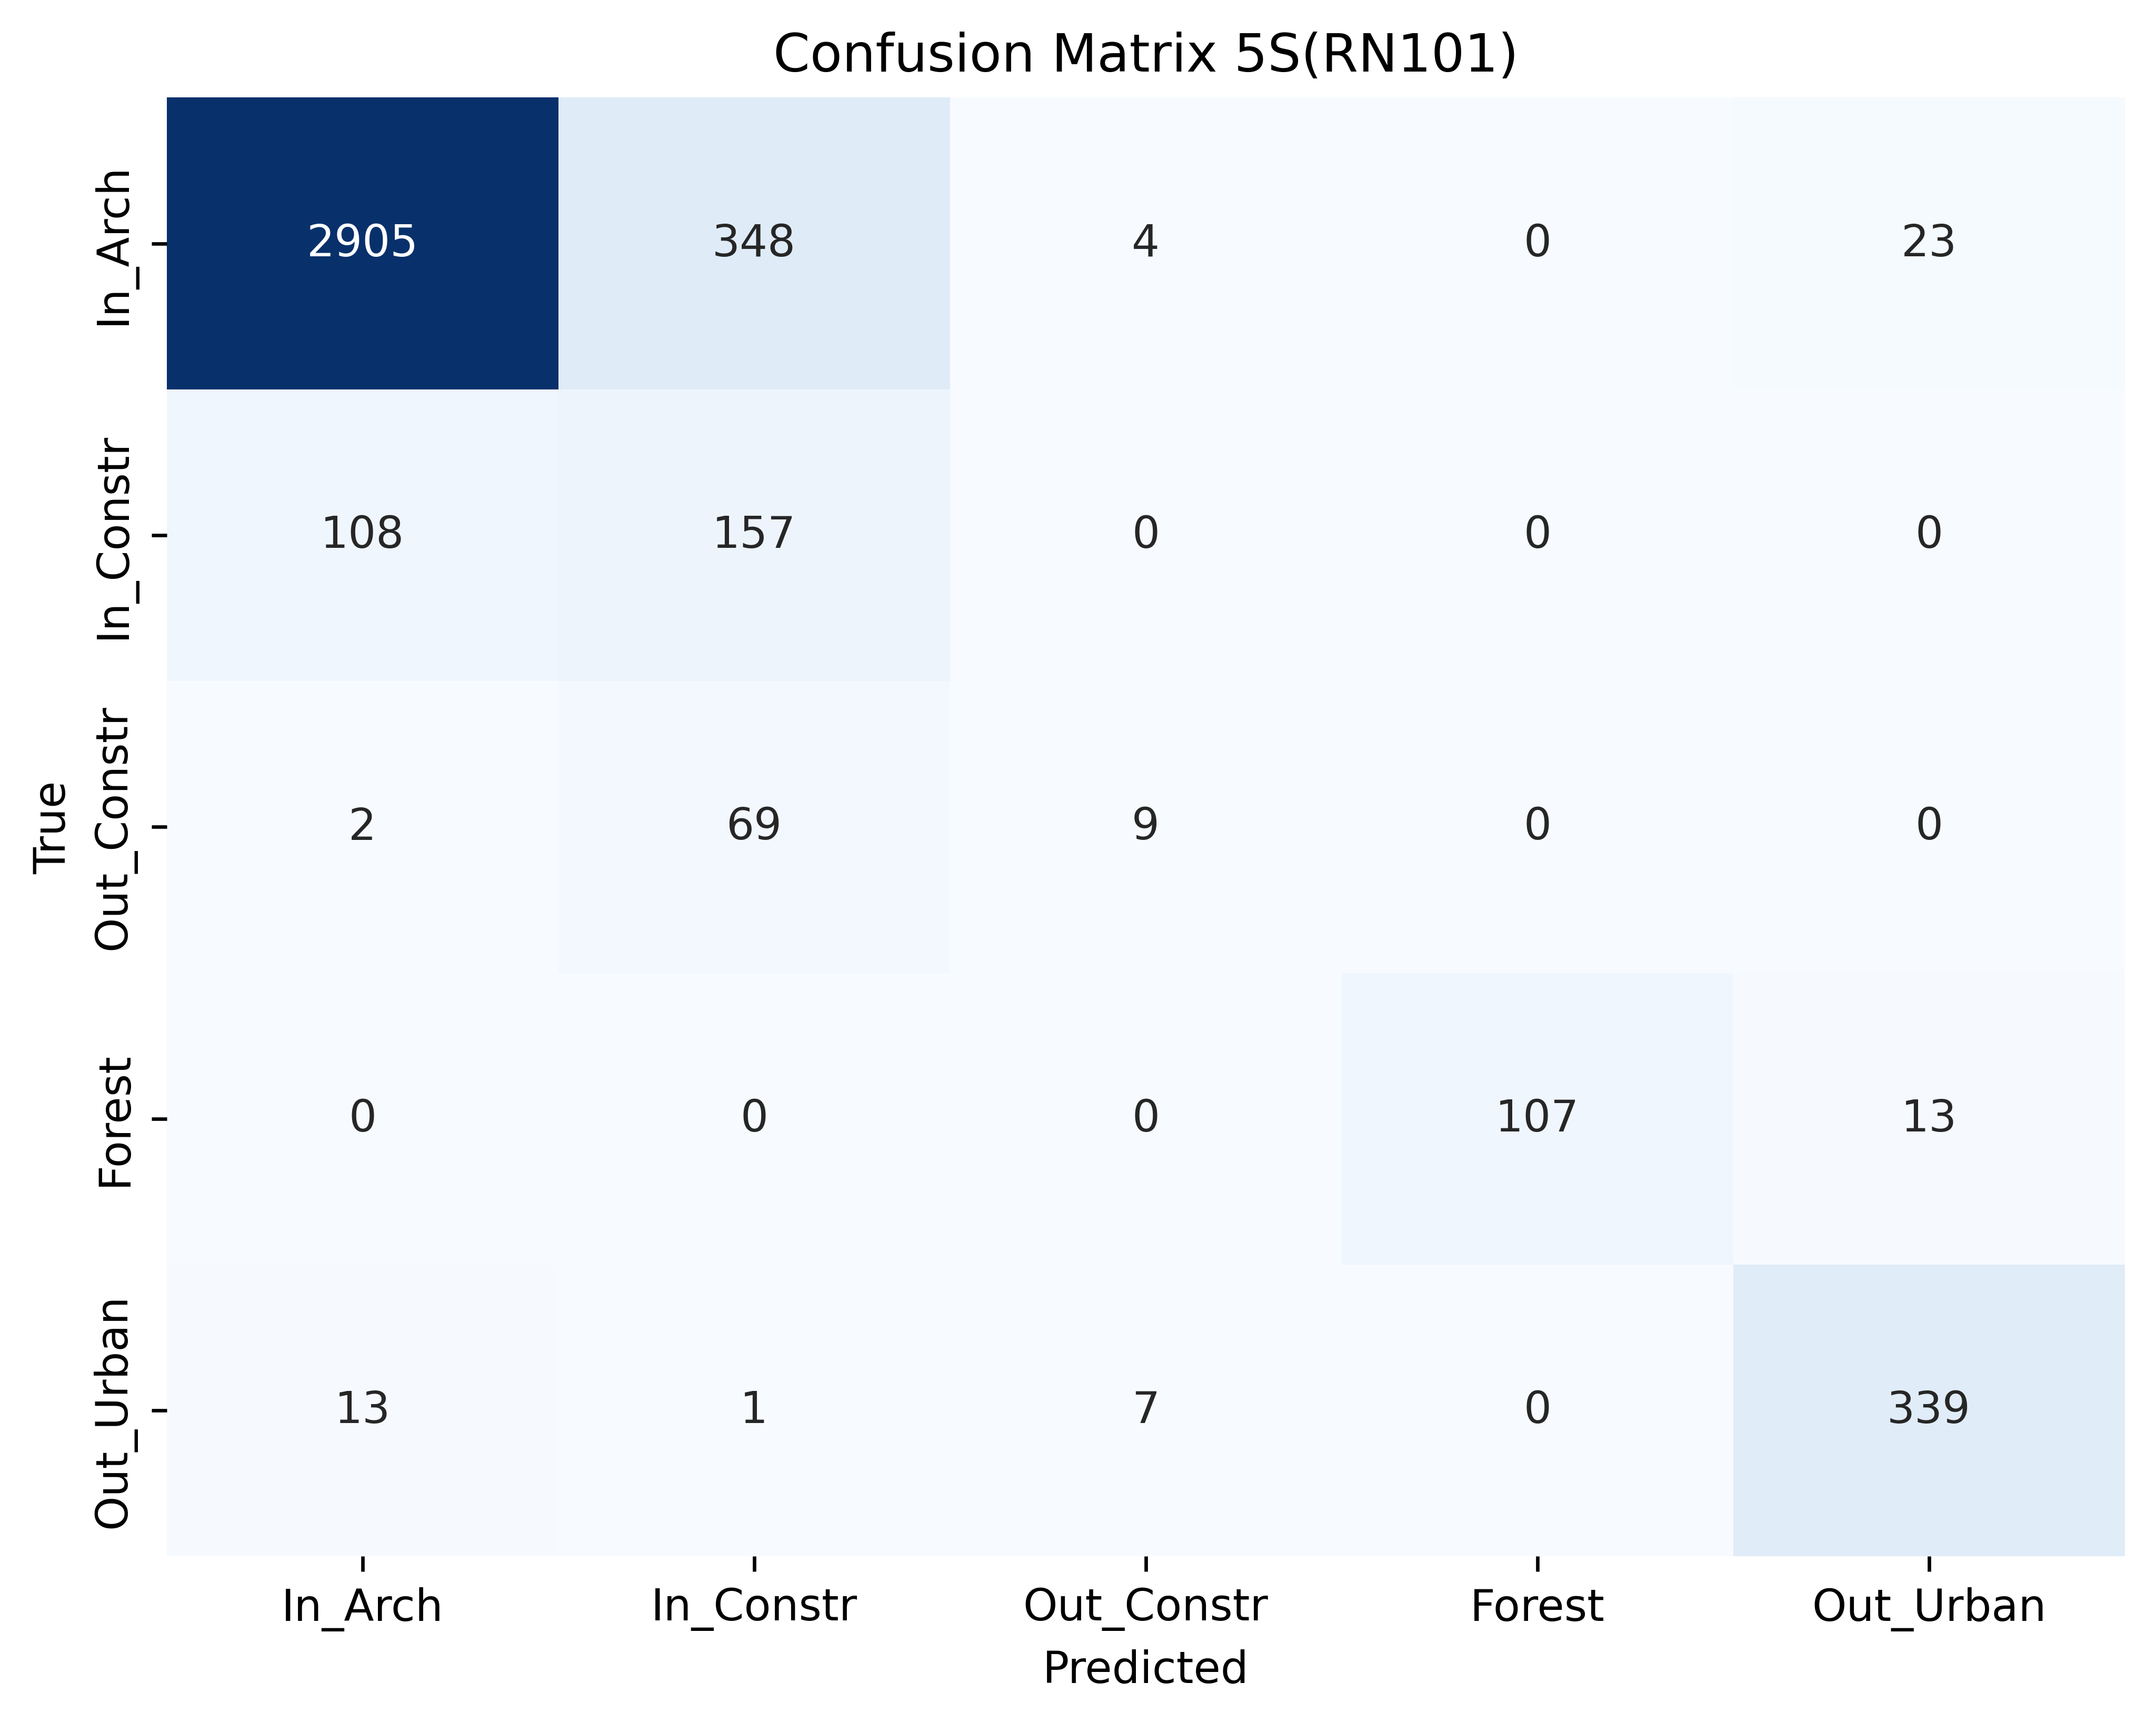
\includegraphics[width=0.45\textwidth]{Images/appendix/resultsRaspi/Confusion Matrix 5S(RN101).png}\label{resultpc:fig:rn50x645s}}
    \caption{Confusion Matrix on Raspberry Pi CPU for CLIP with ResNets as Visual Encoder (5 Sentences as Text Embeddings)}
    \label{resultpc:fig:clipevalraspi5s}
\end{figure}

\begin{figure}[!h]
    \centering
    \subfloat[][TinyClip19M]{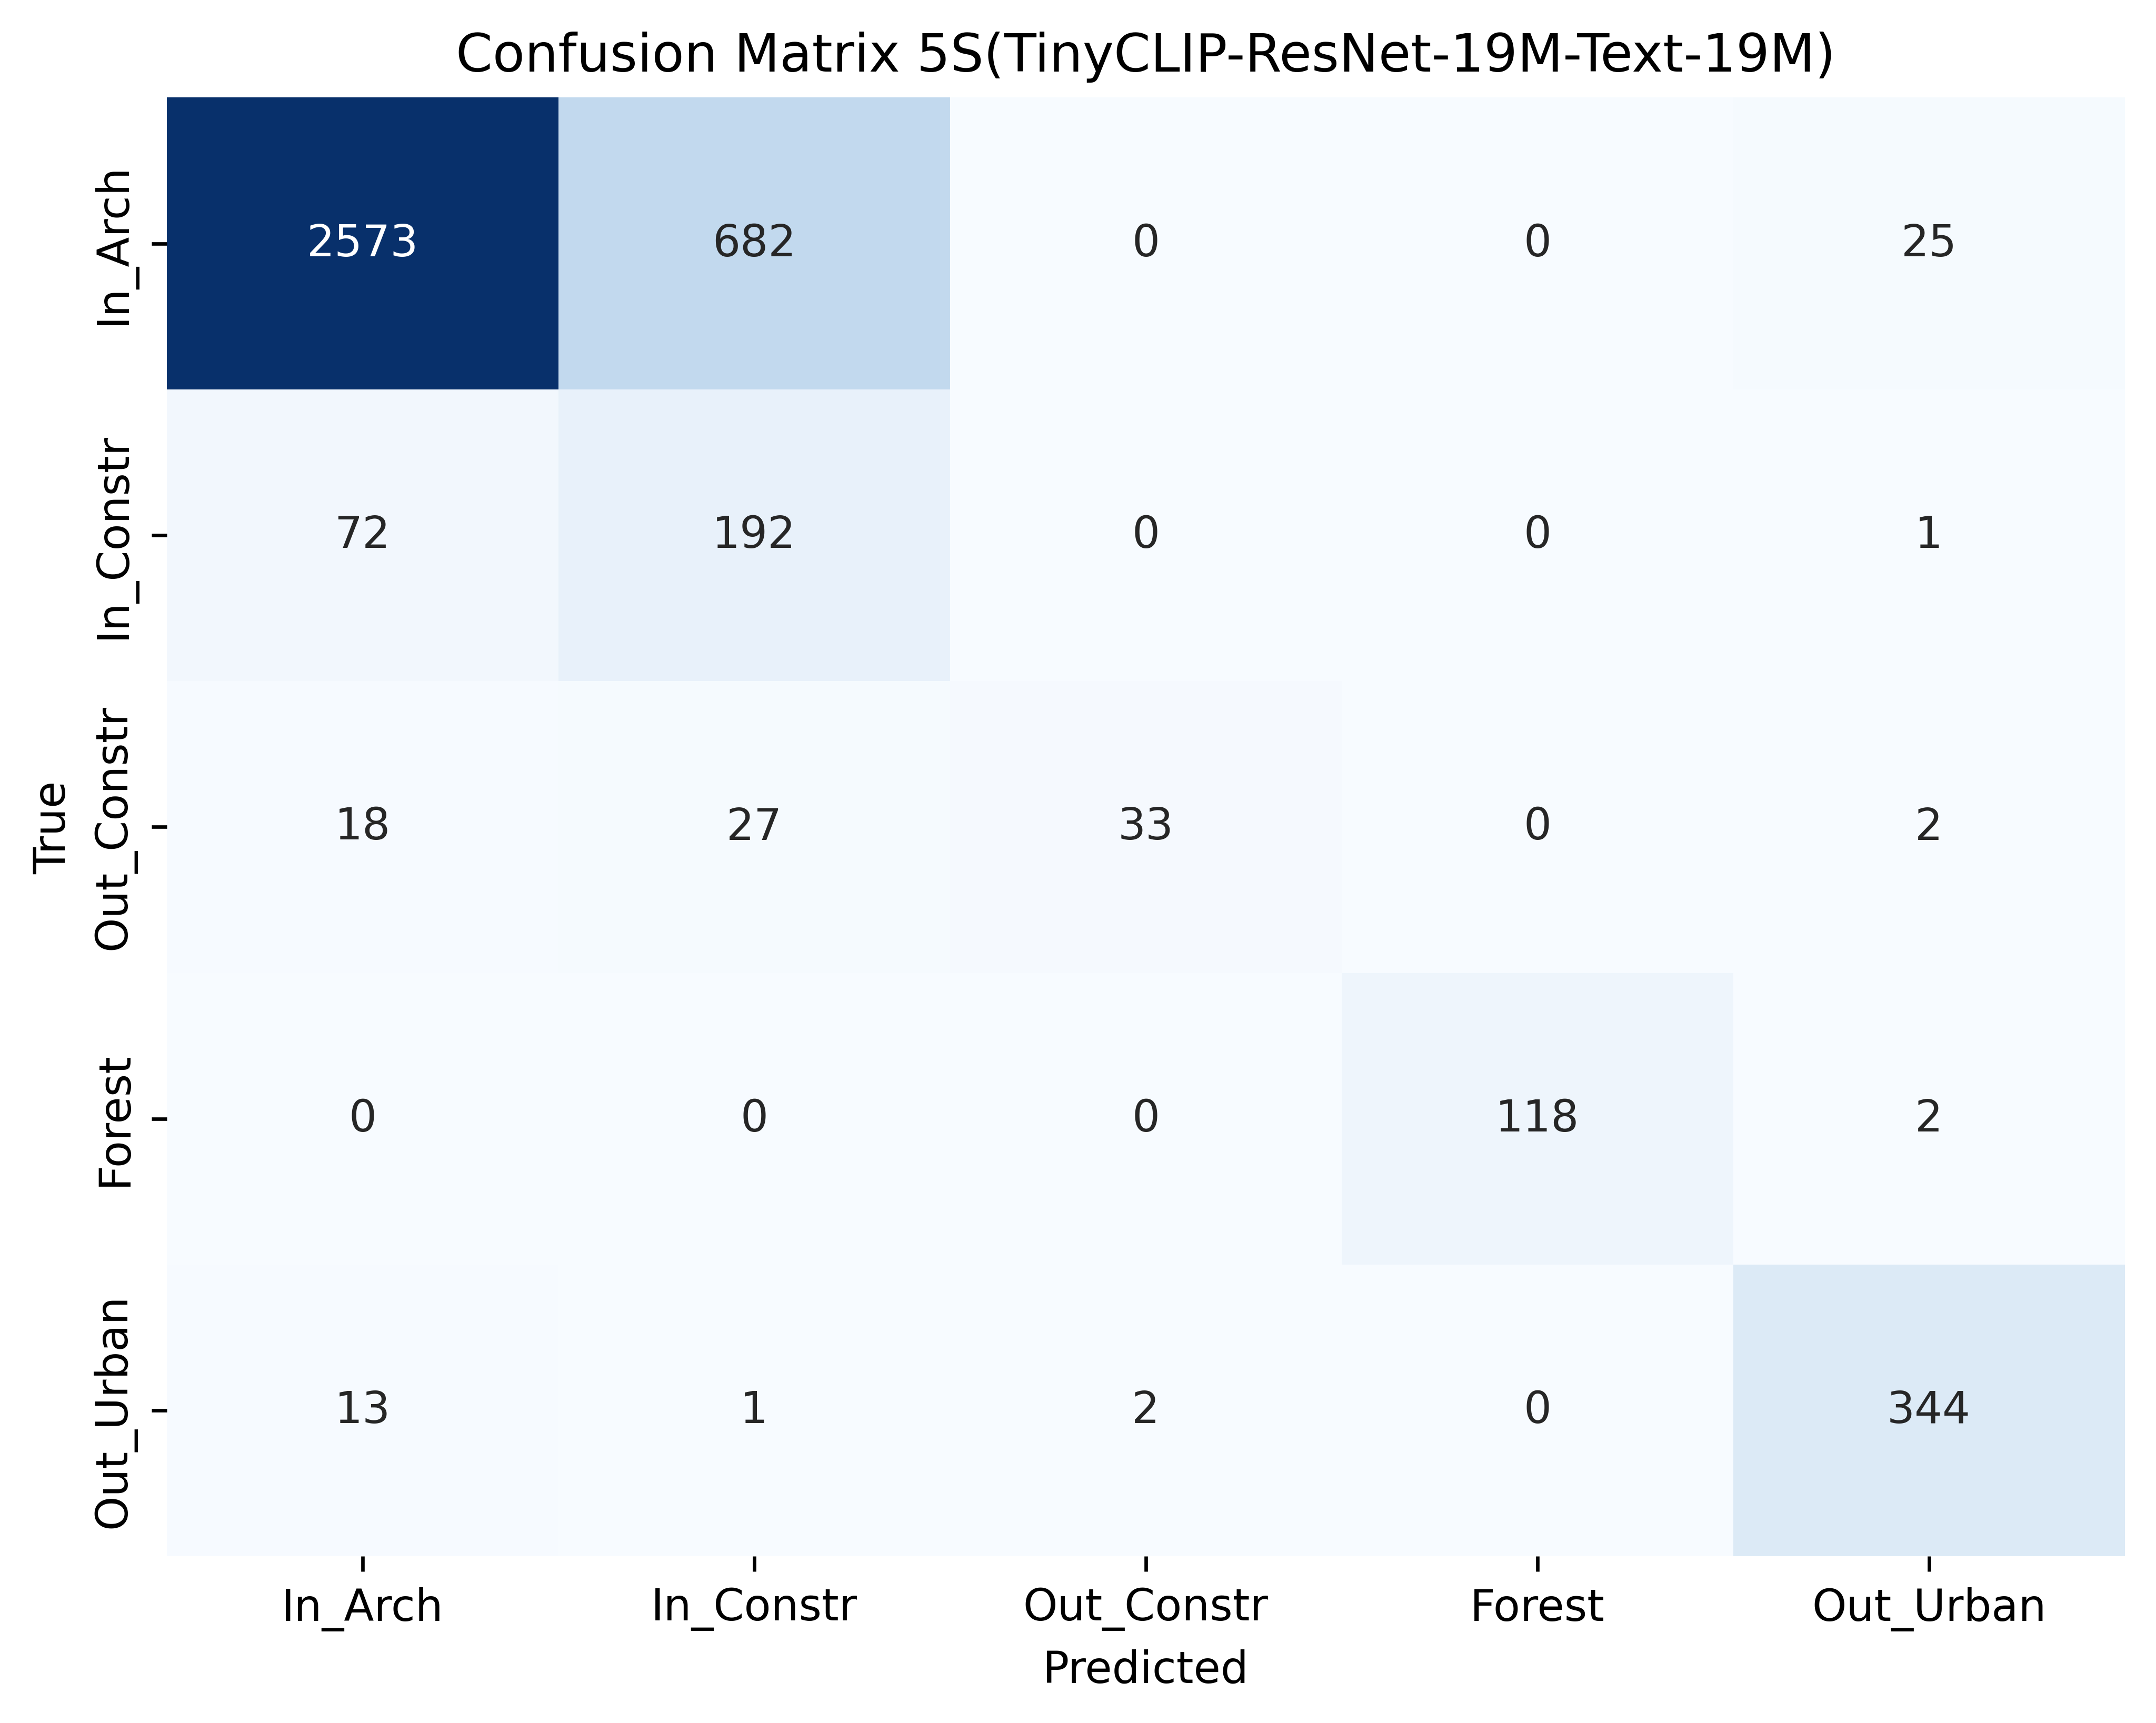
\includegraphics[width=0.45\textwidth]{Images/appendix/resultsRaspi/Confusion Matrix 5S(TinyCLIP-ResNet-19M-Text-19M).png}\label{resultpc:fig:tiny19M5s}}
    \subfloat[][TinyClip30M]{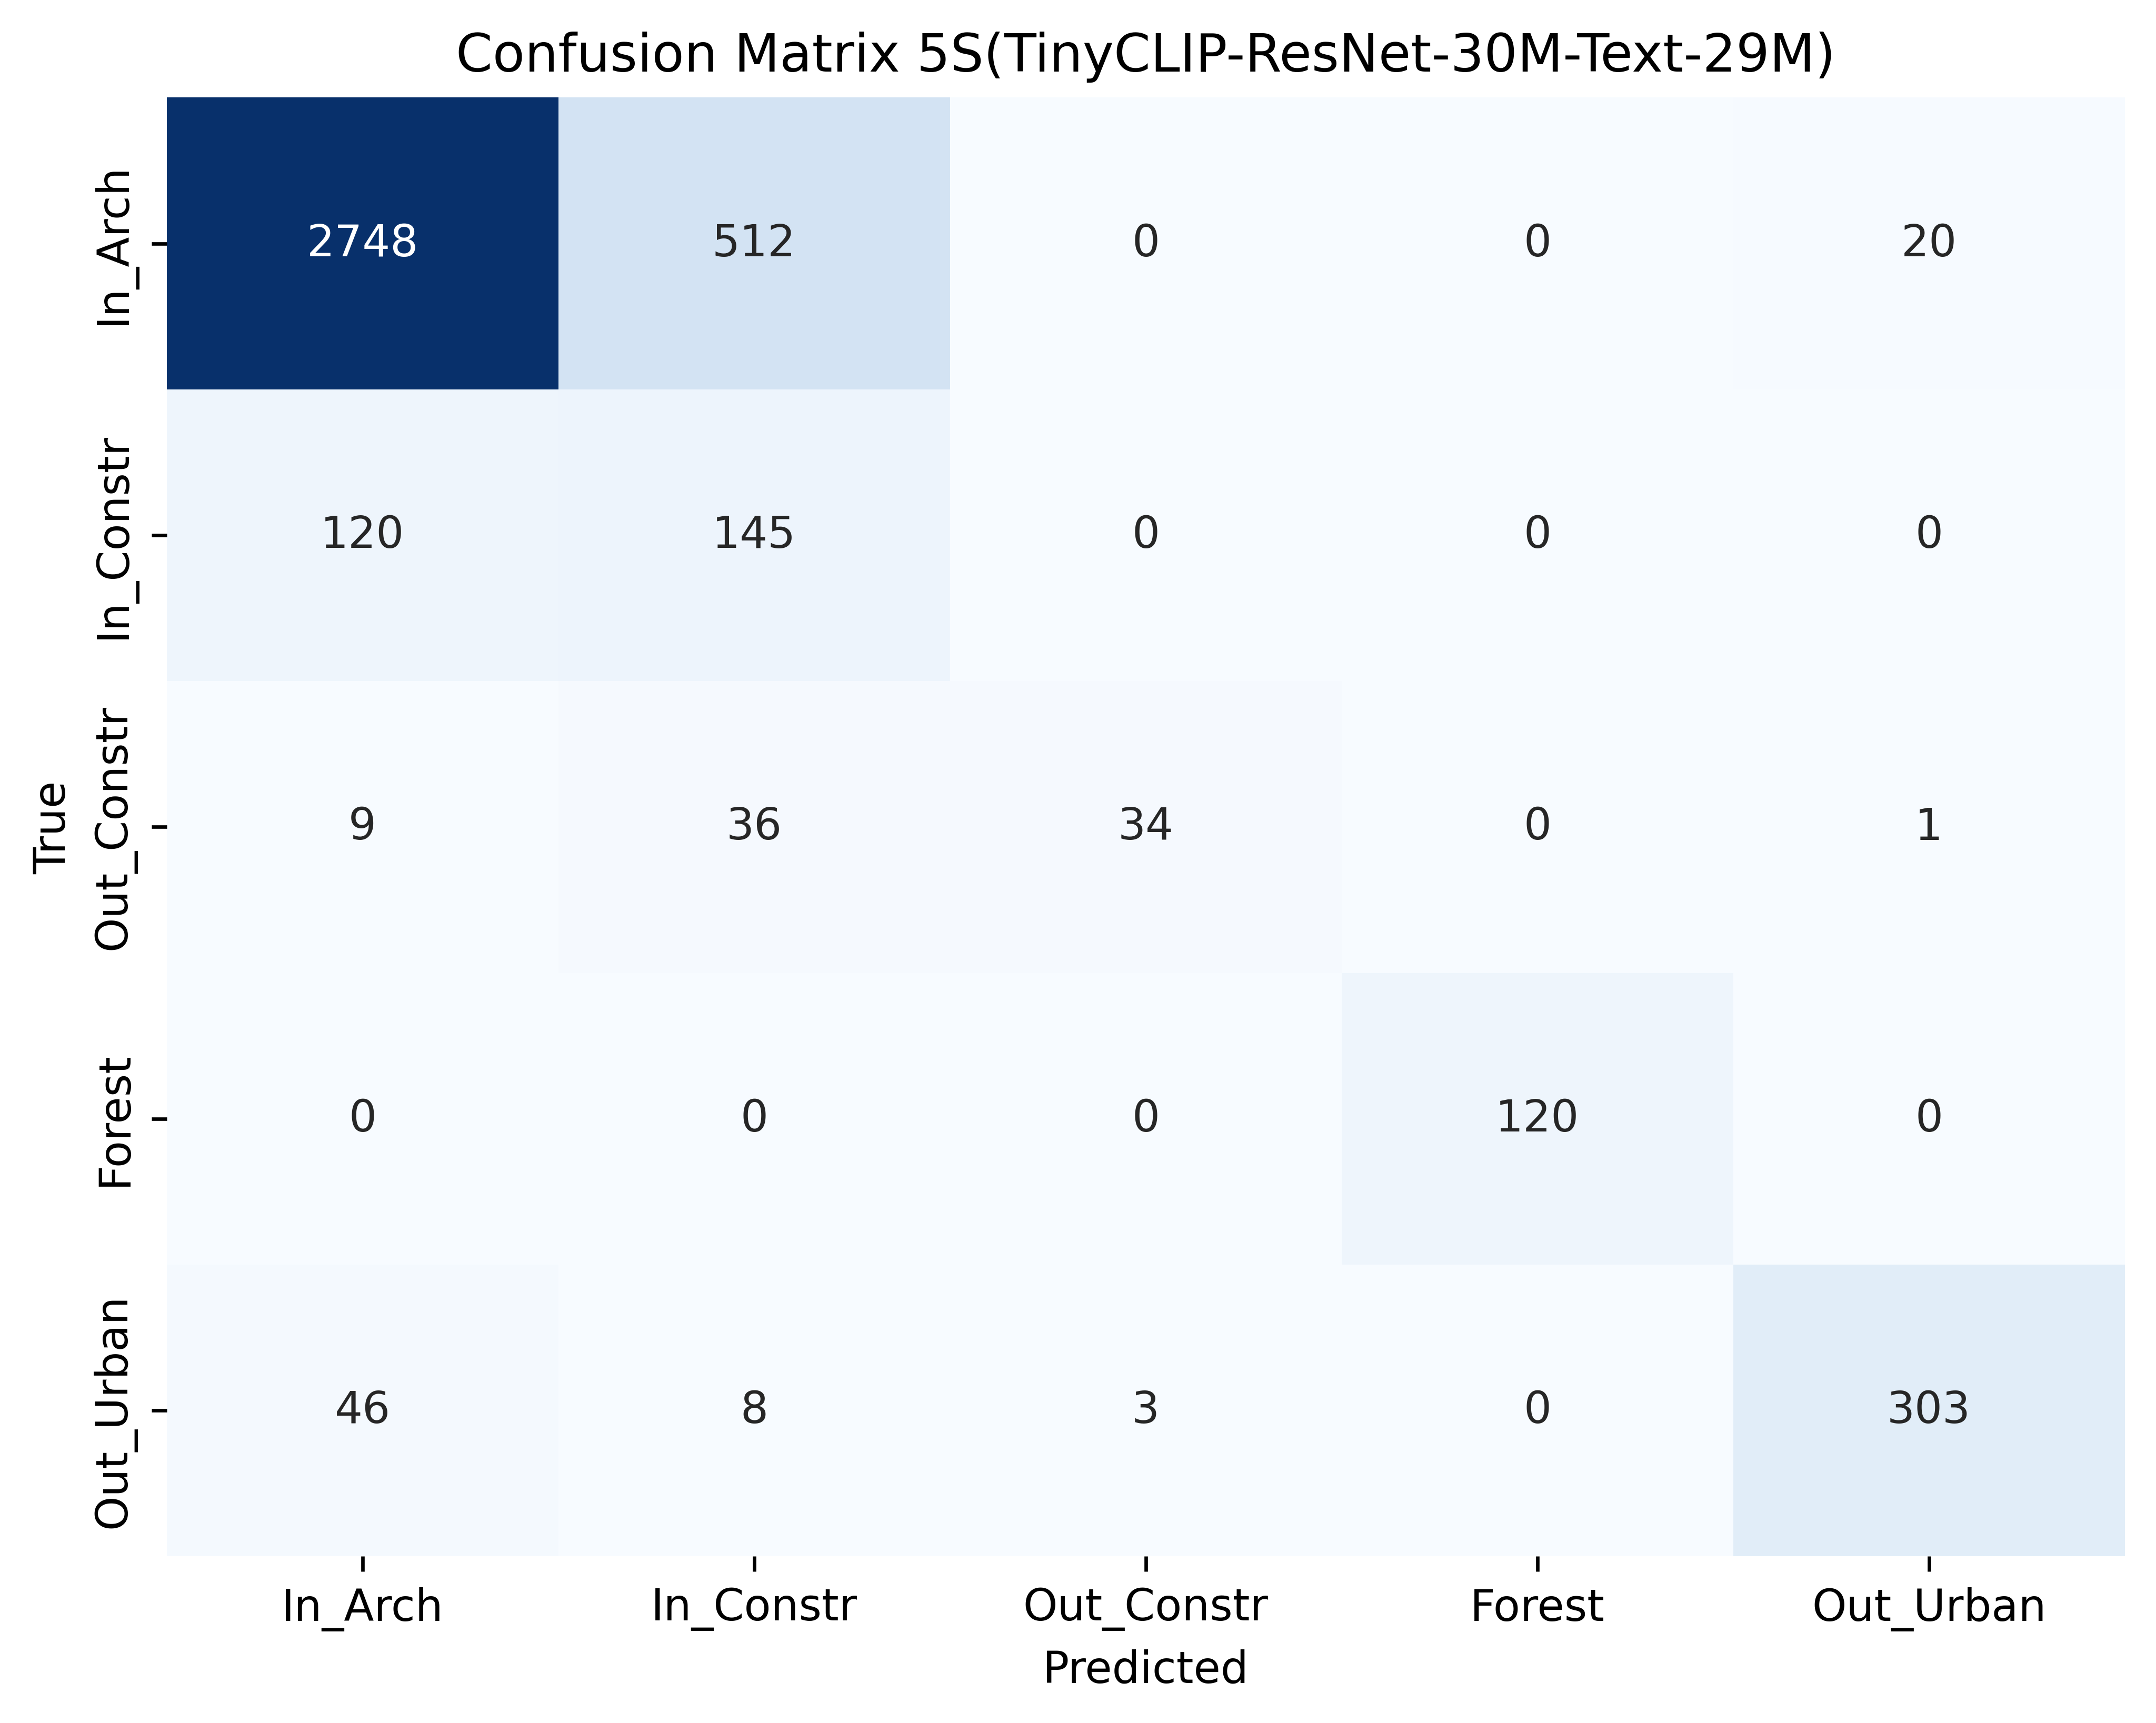
\includegraphics[width=0.45\textwidth]{Images/appendix/resultsRaspi/Confusion Matrix 5S(TinyCLIP-ResNet-30M-Text-29M).png}\label{resultpc:fig:tiny30M5s}}
    \caption{Confusion Matrix on Raspberry Pi CPU for TinyCLIP with ResNets as Visual Encoder (5 Sentences as Text Embeddings)}
    \label{resultpc:fig:tinyclipevalraspi5s}
\end{figure}